\documentclass[chaptersright]{informeutn}
\usepackage{listings}

% Datos del informe
\materia{Dispositivos Electronicos}
\titulo{Trabajo Práctico}
\comision{3R2}
\autores{Santino Noccetti, 405927 - Coordinador\\
         Franco Palombo, 401910 - Documentador/Operario}
\fecha{27/05/2025}

\lstdefinestyle{ltspice}{
  backgroundcolor=\color{gray!10},
  basicstyle=\ttfamily\small,
  keywordstyle=\color{blue},
  commentstyle=\color{green!50!black},
  stringstyle=\color{orange},
  frame=single,
  breaklines=true,
  postbreak=\mbox{\textcolor{red}{$\hookrightarrow$}\space},
  columns=flexible,
  captionpos=b,
  gobble=14
}
\renewcommand{\lstlistingname}{Listado}

\begin{document}

  \maketitle

  \tableofcontents
  \setcounter{page}{1}
  \thispagestyle{plain}

  \chapter{Introduccion}
    En este trabajo practico se divide en el analisis de dos componentes. Por un lado en la simulacion del diodo
    rectificador, se busca visualizar el comportamiento de este y la curva caracteristica para asi comparar el codo de
    conmutacion entre el estado de bloqueo y conduccion que nos presenta el fabricante, luego armar un circuito en el
    laboratorio para poder medir y corroborar lo visto en el simulador. Ademas se incluye en la simulacion el factor de
    la temperatura, para poder ver como afecta al comportamiento.

    Luego se propone un circuito con diodos Zener en CA, para ello se nos exige utilizar el simulador LTspice para
    visualizar su uso para limitar las excursiones de voltaje a niveles deseados. Luego en el laboratorio se nos pide
    armar el mismo circuito para poder visualizar y analizar su uso como recortadores.

  \chapter{Curva caracteristica del Diodo}
    La curva caracteristica del diodo permite establecer una relacion facil de entender entre la corriente que circula
    por el diodo y la caida de tension que se genera. Diferentes diodos tienen diferentes curvas caracteristicas, pero
    casi todas siguen la curva exponencial definida como:

    \begin{equation}
      i_D = I_0 \left(e^{\frac{v_d}{V_T}} - 1 \right)
    \end{equation}

    Las variaciones suelen estar en el termino $I_0$ que es la corriente de polarizacion en inversa, y el termino $V_T$
    que es la variacion de voltaje por grado celsius.

    \section{Polarizacion en directa}
      La polarizacion en directa del diodo implica que la region de empobrecimiento del diodo se contraiga a causa del
      potencial colocado en el diodo. Este potencial, que tiene un flujo de corriente convencional que ingresa por la
      region P y egresa por la region N (en flujo no convencional, los $e^-$ ingresan por N y egresan por P). Este
      flujo de corriente provoca que haya un exceso de portadores mayoritarios en la region P, haciendo que aquellos
      que tienen suficiente energia potencial puedan sobrepasar la region de empobrecimiento, recombinandose con los
      portadores mayoritarios de la region N y generando un movimiento de cargas. Esto pasa tambien en la region N.

      A medida que mas portadores mayoritarios fluyen, mas se contrae la region de empobrecimiento, causando que los
      portadores mayoritarios requieran menos potencial para sobrepasar la barrera. Este fenomeno es por el cual el
      diodo va teniendo menos "resistencia equivalente" a medida que el voltaje o la corriente aumentan.

      \subsection{Diodo de Silicio}
        Para corroborar la curva caracteristica del diodo de silicio, y como esta responde a los cambios de voltaje y
        temperatura, se creo un circuito en el software LTSpice muy basico para probar la polarizacion del diodo de
        silicio.

        El programa, de manera automatica, genera un barrido de tension que arranca en los $-2V$ y termina en los $10V$,
        haciendo pasos de $100mV$ por muestra. De esta forma hay suficiente resolucion para considerarla una buena
        aproximacion de la curva caracteristica del diodo.

        Se selecciono el diodo 1N4007 como diodo de pruebas de silicio y $R_1 = 1K\Omega$. El circuito armado en
        LTSpice se puede ver en figura (\ref{crkt.Si.directa}) y se han empleado las directivas mostradas en el
        listado (\ref{list.Si.directa}).
        \begin{figure}[H]
          \centering
          \begin{minipage}{0.45\textwidth}
            \begin{circuitikz}[american voltages]
              \draw (0, -1) to [V=$V_1$, invert]             (0, 3)
                            to [short, -, i>^=$I_t$]         (1, 3)
                            to [R=$R_1$, v=$V_{R_1}$]        (4, 3)
                            to [short, -]                    (5, 3)
                            to [D=$1N4007$, v=$V_{D}$]       (5, -1)
                            to [short, -]                    (5, -1)
                            to [short, -]                    (0, -1)
                            ;
            \end{circuitikz}
            \caption{Circuito con diodo de silicio 1N4007.}
            \label{crkt.Si.directa}
          \end{minipage}
          \hfill
          \begin{minipage}{0.45\textwidth}
            \begin{lstlisting}[style=ltspice, caption={Parámetros de simulación LTspice}]
              .dc V1 -2 10 100m
            \end{lstlisting}
            \label{list.Si.directa}
          \end{minipage}
        \end{figure}

        Habiendo simulado el circuito anterior, se extrayeron los resultados para ser mostrados en la figura
        (\ref{graph.simulation.Si.directa}).

        \begin{figure}[!ht]
          \centering
          \begin{minipage}{0.45\textwidth}
            \begin{tikzpicture}
              \begin{axis}[
                xlabel={$V$ [V]},
                ylabel={$I$ [mA]},
                grid=both,
                minor tick num=1,
                extra x ticks={0.7},
                extra x tick style={
                  grid style={red, thick, dashed},
                  tick style={red},
                  tick label style={red}
                 },
                scaled ticks=false,
                restrict x to domain=-1:4,
              ]
              \addplot[
                color=blue,
                mark=none,
                thick,
              ] table[
                col sep=tab,
                header=true,
                x=V1,
                y expr=\thisrow{I(D1)}*1000
              ] {simulations/TP2_1_graph.txt};
              \end{axis}
            \end{tikzpicture}
            \caption{Grafico de la curva caracteristica del simulador}
            \label{graph.simulation.Si.directa}
          \end{minipage}
          \hfill
          \begin{minipage}{0.45\textwidth}
            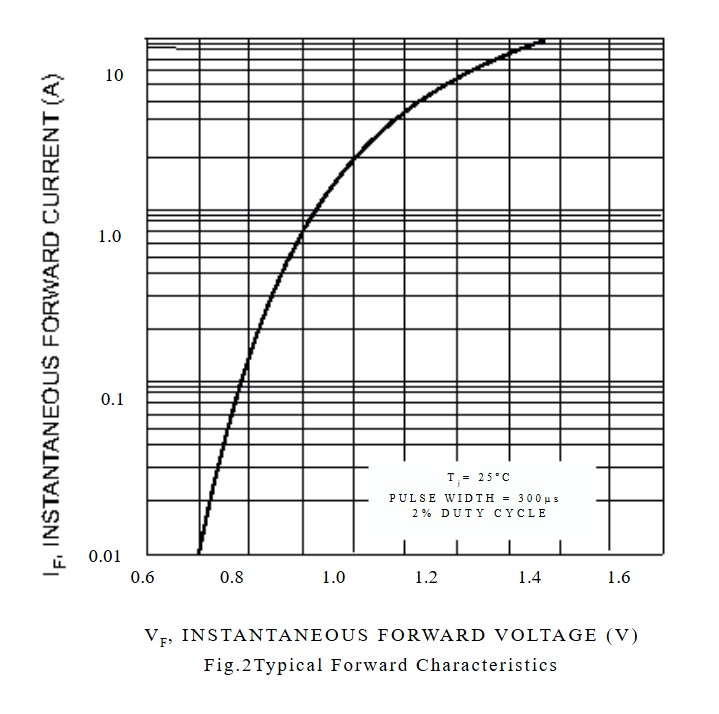
\includegraphics[width=1\textwidth]{pictures/Curva_Datash_Si.jpg}
            \caption{Grafico de la curva caracteristica de la hoja de datos.}
            \label{graph.datasheet.Si.directa}
          \end{minipage}
        \end{figure}

        Se puede observar que los graficos son significativamente diferentes uno del otro. Esto se debe a que el
        analisis de baja corriente/voltaje que se esta haciendo para este trabajo practico no suele ser importante
        (por lo menos para el diodo seleccionado) debido a que el rango operativo esta a mas de 100 veces la corriente
        (por eso la escala es logaritmica) a la que se sometido el diodo en la simulacion.

        De todas formas, se puede apreciar que el "codo de conmutacion" efectivamente ocurre a los 0.7V en ambas
        graficas. Lo que podemos apreciar con mayor presicion en el grafico simulado es la curva de corriente la cual
        el diodo experimenta cuando pasa de no estar polarizado a cuando conduce. En la grafica del fabricante, se
        puede apreciar mucho mejor, como es que lo que se ve en la simulacion como una rampa lineal, en altas
        corrientes en realidad no es tan lineal, y empieza a experimentar un aumento de la "resistencia equivalente"
        debido a la proximidad con el limite operativo del diodo.

      \subsection{Diodo de Germanio}
        A continuacion se presenta el circuito utilizado en LTspice para visualizar la curva caracteristica del
        diodo de Germanio.

        La configuracion utilizada fue:
        \begin{itemize}
          \item Una fuente DC que realiza un barrido lineal de 100$mV$ desde -2 $V$ hasta los 10 $V$ 
          \item Resistencia de 1$k$
          \item Diodo 1N60
        \end{itemize}

        \begin{figure}[h]
          \centering
          \begin{minipage}{0.7\textwidth}
            \centering
            \begin{circuitikz}[american voltages]
              % nodos
              \draw
              (0, -1) to [V=$V_1$, invert]           (0, 3)
                      to [short, -, i>^=$I_t$]       (1, 3)
                      to [R=$R_1$, v=$V_{R_1}$]      (4, 3)
                      to [short, -]                  (5, 3)
                      to [D=$1N60$, v=$V_{D}$]       (5, -1)
                      to [short, -]                  (5, -1)
                      to [short, -]                  (0, -1)
                      ;
            \end{circuitikz}
          \end{minipage}
          \centering
          \caption{Circuito con diodo de Germanio}
        \end{figure}

        Comparacion del grafico obtenido en el simulador con el proporcionado en la hoja de datos del fabricante
        Diode Semiconductor Korea:

        \begin{figure}[!h]
          \centering
          \begin{minipage}[b]{0.4\textwidth}
            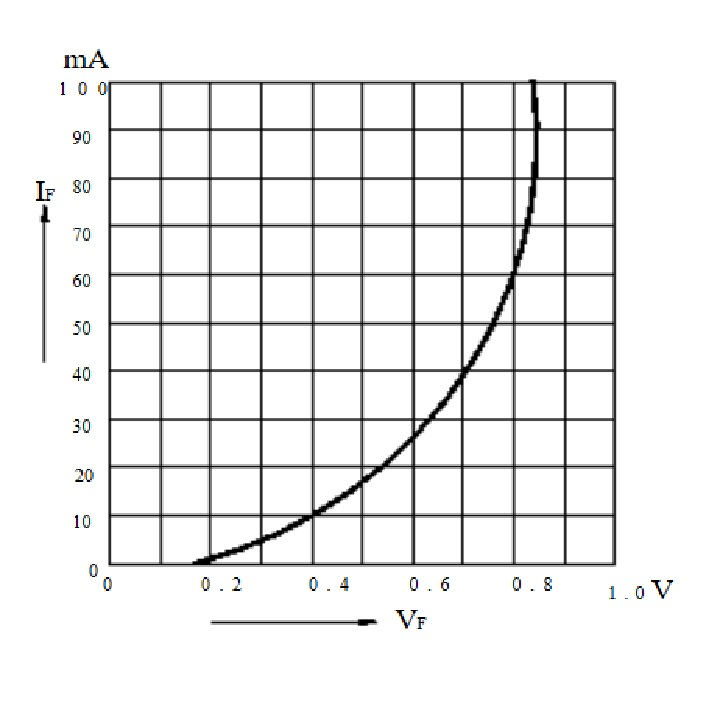
\includegraphics[width=1.1\linewidth]{pictures/Curva_Datash_Ge.jpg}
            \caption{Grafico de la curva del simulador}
          \end{minipage}
          \hfill
          \begin{minipage}[b]{0.4\textwidth}
            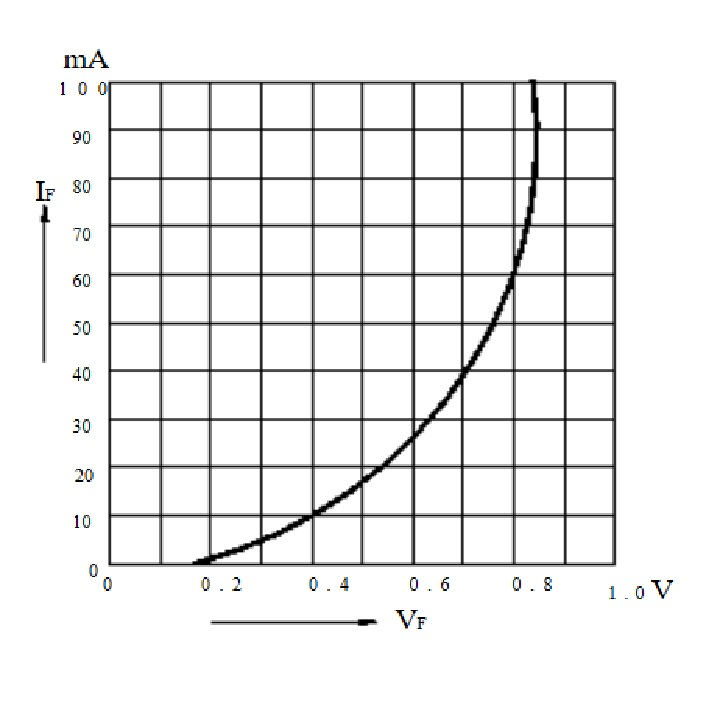
\includegraphics[width=1.1\linewidth]{pictures/Curva_Datash_Ge.jpg}
            \caption{Grafico de la curva del Datasheet}
          \end{minipage}
        \end{figure}

        Al igual que en el diodo de Silicio, este mantiene claras igualdades en la curva caracteristica del diodo
        comparandola con la hoja de datos del fabricante.

      \subsection{Comparacion de ambas simulaciones}

        \begin{figure}[!h]
          \centering
          \begin{minipage}[b]{0.4\textwidth}
            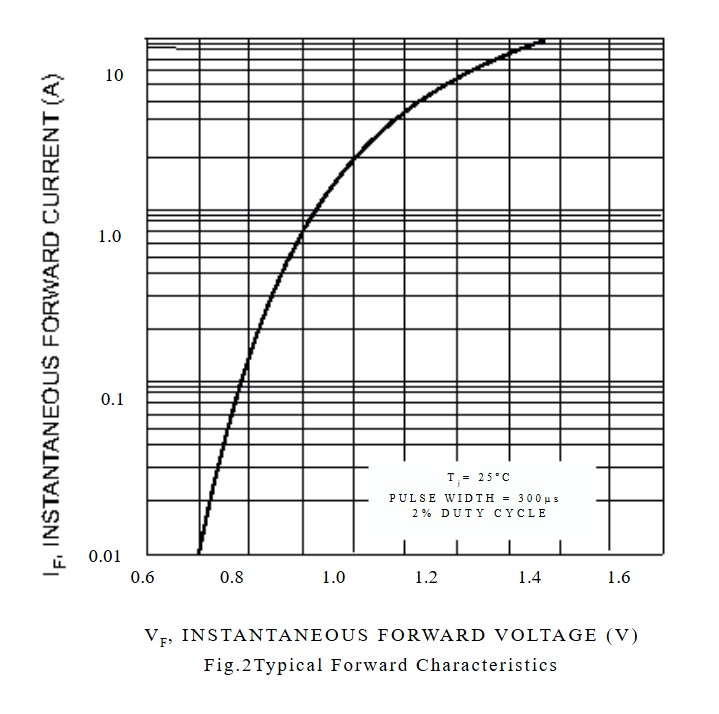
\includegraphics[width=1.1\linewidth]{pictures/Curva_Datash_Si.jpg}
            \caption{Grafico de la curva del simulador}
          \end{minipage}
        \end{figure}

        Cuando se observa de esta forma ambas curvas se logra apreciar una clara diferencia en cuanto al voltaje
        necesario para lograr poner los diodos en conduccion, siendo la de Germanio alrededor de los $0.2V$ y $0.3V$
        mientras que el de Silicio se encuentra entre $0.6V$ y $0.7V$.Esta diferencia en el codo de conmutacion se
        debe principalmente a la diferencia de energia necesaria para que los electrones pasen de la banda de
        valencia a la banda de conduccion, a su vez tambien se le atribuye a que el Germanio posee mayor corriente de
        fuga, generando asi que la curva se pronuncie mucho antes que la del Silicio. Esto tiene implicaciones a la
        hora de elegir que tipo de diodo usar, ya que el de Germanio se utiliza para circuitos con poco voltaje, sin
        embargo, el de Silicio es el mas utilizado ya que posee menor corriente de fuga y mayor estabilidad a los
        cambios de temperatura.

    \section{Polarizacion en inversa}
      \subsection{Diodo de silicio}
        A continuacion se presenta el circuito utilizado en LTspice para visualizar la curva caracteristica del diodo de Silicio en inversa.

        \begin{itemize}
          \item Una fuente DC que realiza un barrido lineal de 100$mV$ desde -2 $V$ hasta los 1200 $V$ 
          \item Resistencia de 1$k$
          \item Diodo 1N4007
        \end{itemize}
        \begin{figure}[h]
          \centering
          \begin{minipage}{0.7\textwidth}
            \centering
            \begin{circuitikz}[american voltages]
              % nodos
              \draw
              (0, -1) to [V=$V_1$, invert]          (0, 3)
                      to [short, -, i>^=$I_t$]              (1, 3)
                      to [R=$R_1$, v=$V_{R_1}$]             (4, 3)
                      to [short, -]                         (5, 3)
                      to [D=$1N4007$, v=$V_{D}$]            (5, -1)
                      to [short, -]                         (5, -1)
                      to [short, -]                         (0, -1)
                      ;
            \end{circuitikz}
          \end{minipage}
          \centering
          \caption{Circuito con diodo de Silicio en inversa}
        \end{figure}

        \begin{figure}[!h]
          \centering
          \begin{minipage}[b]{0.4\textwidth}
            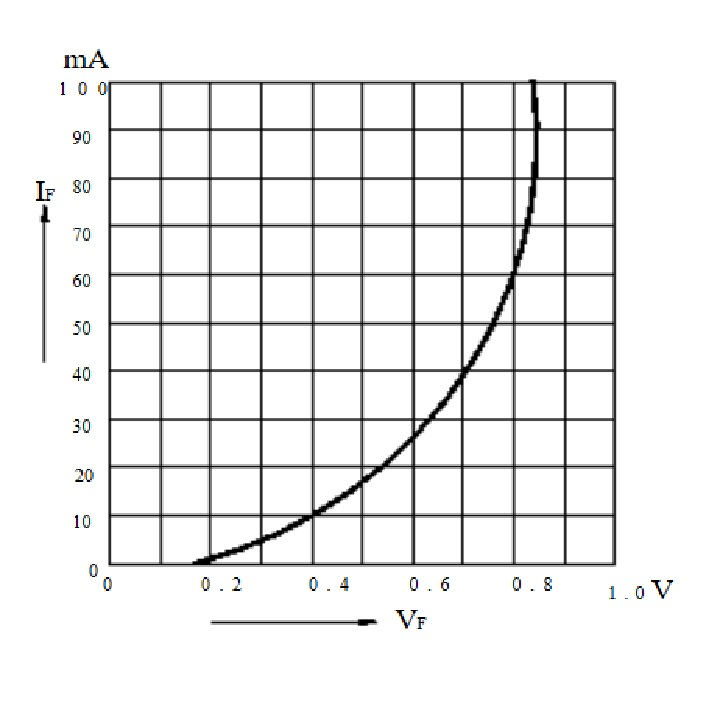
\includegraphics[width=1.1\linewidth]{pictures/Curva_Datash_Ge.jpg}
            \caption{Grafico de la curva del diodo de Silicio en inversa}
          \end{minipage}
        \end{figure}

      \subsection{Diodo de Germanio}
        A continuacion se presenta el circuito utilizado en LTspice para visualizar la curva caracteristica del diodo
        de Germanio en inversa.

        \begin{itemize}
          \item Una fuente DC que realiza un barrido lineal de 100$mV$ desde -2 $V$ hasta los 45 $V$ 
          \item Resistencia de 1$k$
          \item Diodo 1N60
        \end{itemize}
        \begin{figure}[h]
          \centering
          \begin{minipage}{0.7\textwidth}
            \centering
            \begin{circuitikz}[american voltages]
              % nodos
              \draw
                  (0, -1) to [V=$V_1$, invert]           (0, 3)
                          to [short, -, i>^=$I_t$]       (1, 3)
                          to [R=$R_1$, v=$V_{R_1}$]      (4, 3)
                          to [short, -]                  (5, 3)
                          to [D=$1N4007$, v=$V_{D}$]     (5, -1)
                          to [short, -]                  (5, -1)
                          to [short, -]                  (0, -1)
                          ;
            \end{circuitikz}
          \end{minipage}
          \centering
          \caption{Circuito con diodo de Germanio en inversa}
        \end{figure}

        \begin{figure}[!h]
          \centering
          \begin{minipage}[b]{0.4\textwidth}
            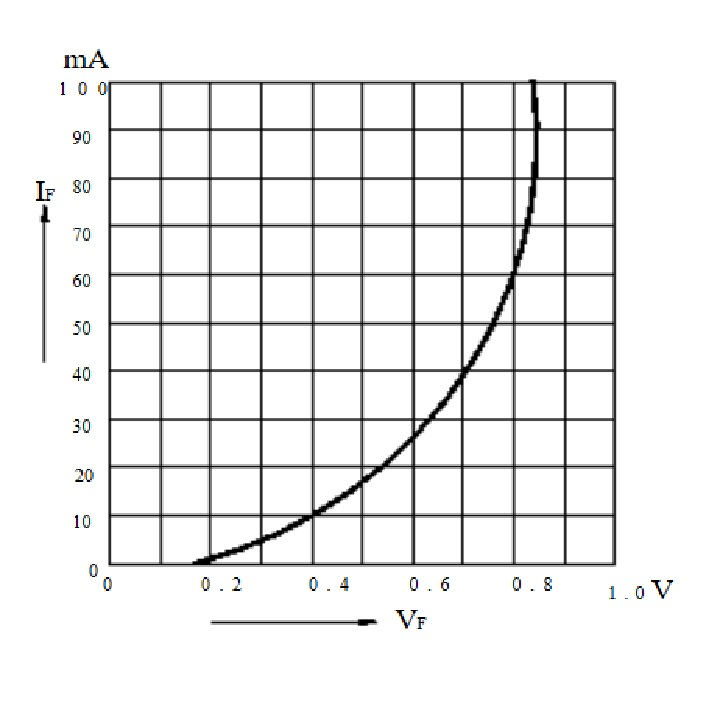
\includegraphics[width=1.1\linewidth]{pictures/Curva_Datash_Ge.jpg}
            \caption{Grafico de la curva del diodo de Germanio en inversa}
          \end{minipage}
        \end{figure}

        Conociendo los datos que nos brinda el fabricante, sabemos que la tension inversa maxima es de 45$V$, por lo
        tanto se llega a observar que cerca de ese valor el diodo tiende a la region Zenner.

  \chapter{Actividad de laboratorio}
    Se pide poner en practica y corroborar los datos conseguidos en el simulador y armar el mismo circuito
    propuesto y anotar los valores conseguidos.

      \subsection{Diodo de Silicio}

  \part{Comportamiento del diodo en función de la temperatura}
    \chapter{Actividad de simulacion}
  \part{Circuitos recortadores con diodos Zener}
    \chapter{Actividad de simulacion}
    \chapter{Actividad de laboratorio}
    \chapter{Analisis sobre parametros de hoja de datos}
\end{document}
